\section{Examples of model application}
\label{sec:Examples of model applicatio}

To improve understanding of our data and the models we show some application of the models on some exemplary fridges. We choose fridges 4 and 24. Hence $f \in \left\{4,24\right\}$. Furthermore we start with analysing the aggregated 4 main categories which means $K=4$. 

We first begin with plotting the values of time series. The x-axis shows the time and the y-axis the number of units sold. Since we have four main categorie for each fridge, we have four subplots. 

\begin{figure}[htb]
\centering
\begin{subfigure}[b]{0.45\textwidth}
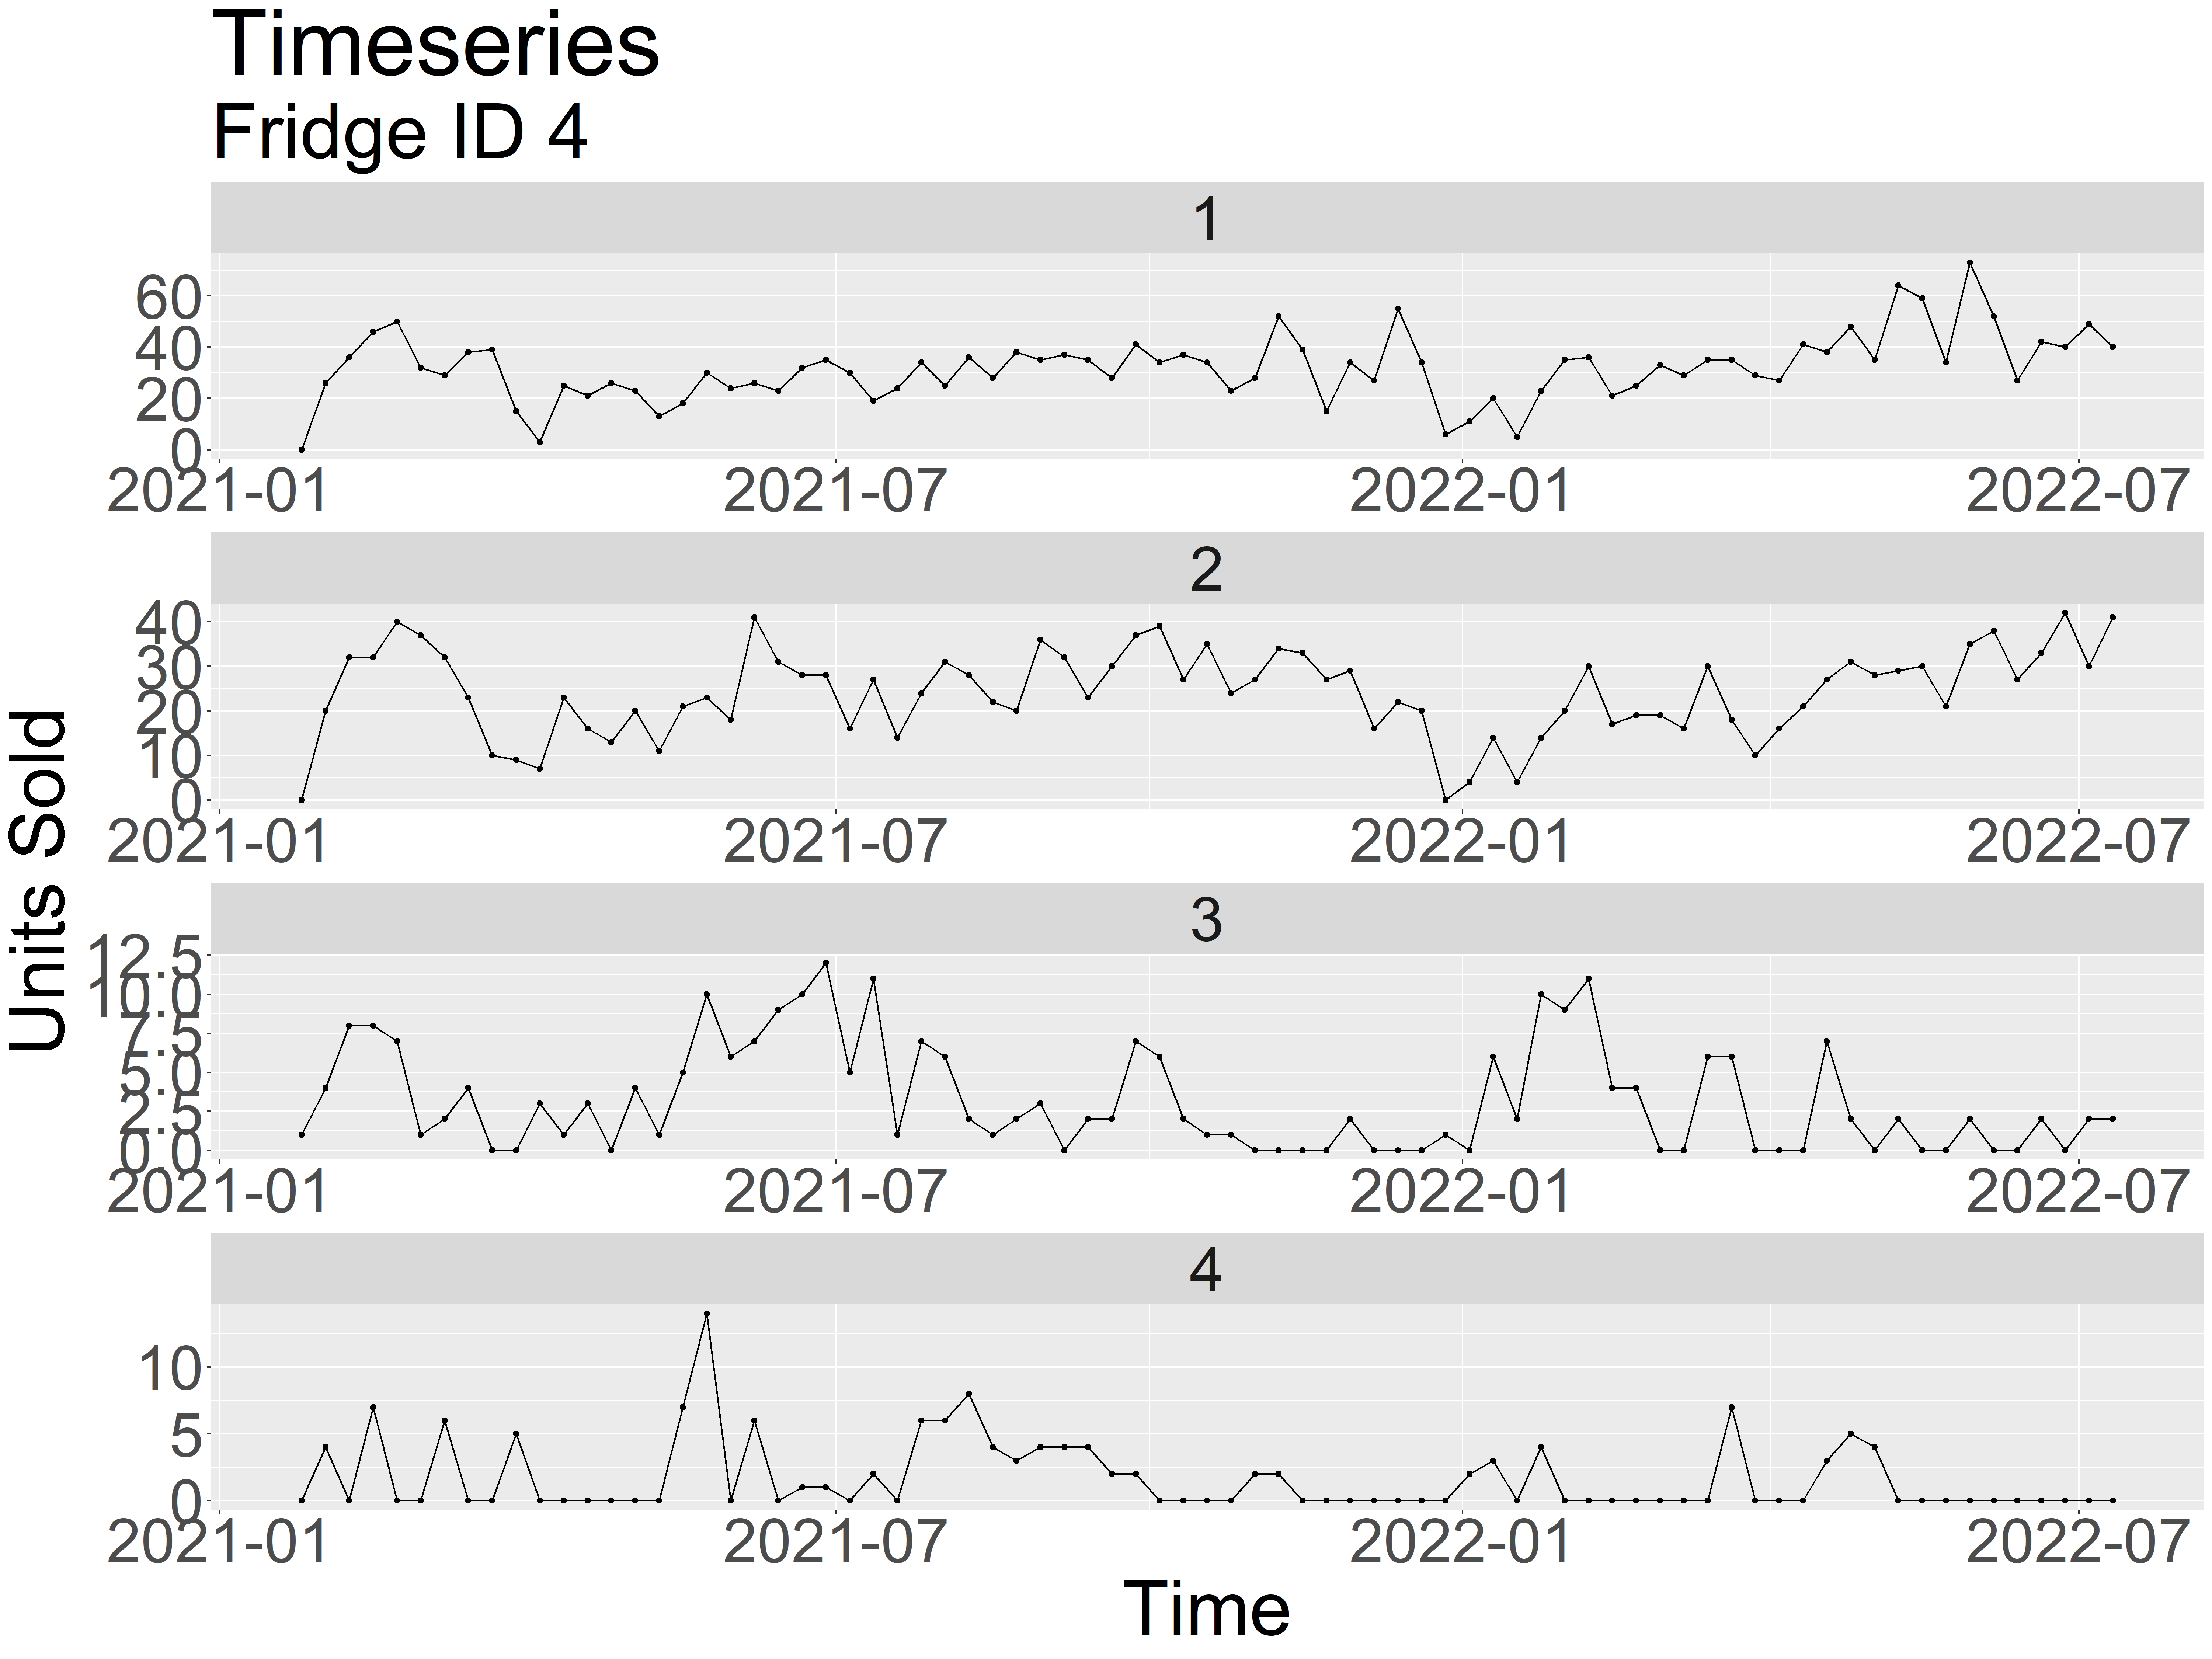
\includegraphics[width=\textwidth]{Raw_Timeseries_ID4.png} 
\caption{Fridge 4 with all four main categories}
\label{fig:TS Fridge 4}
\end{subfigure}
\hfill
\begin{subfigure}[b]{0.45\textwidth}
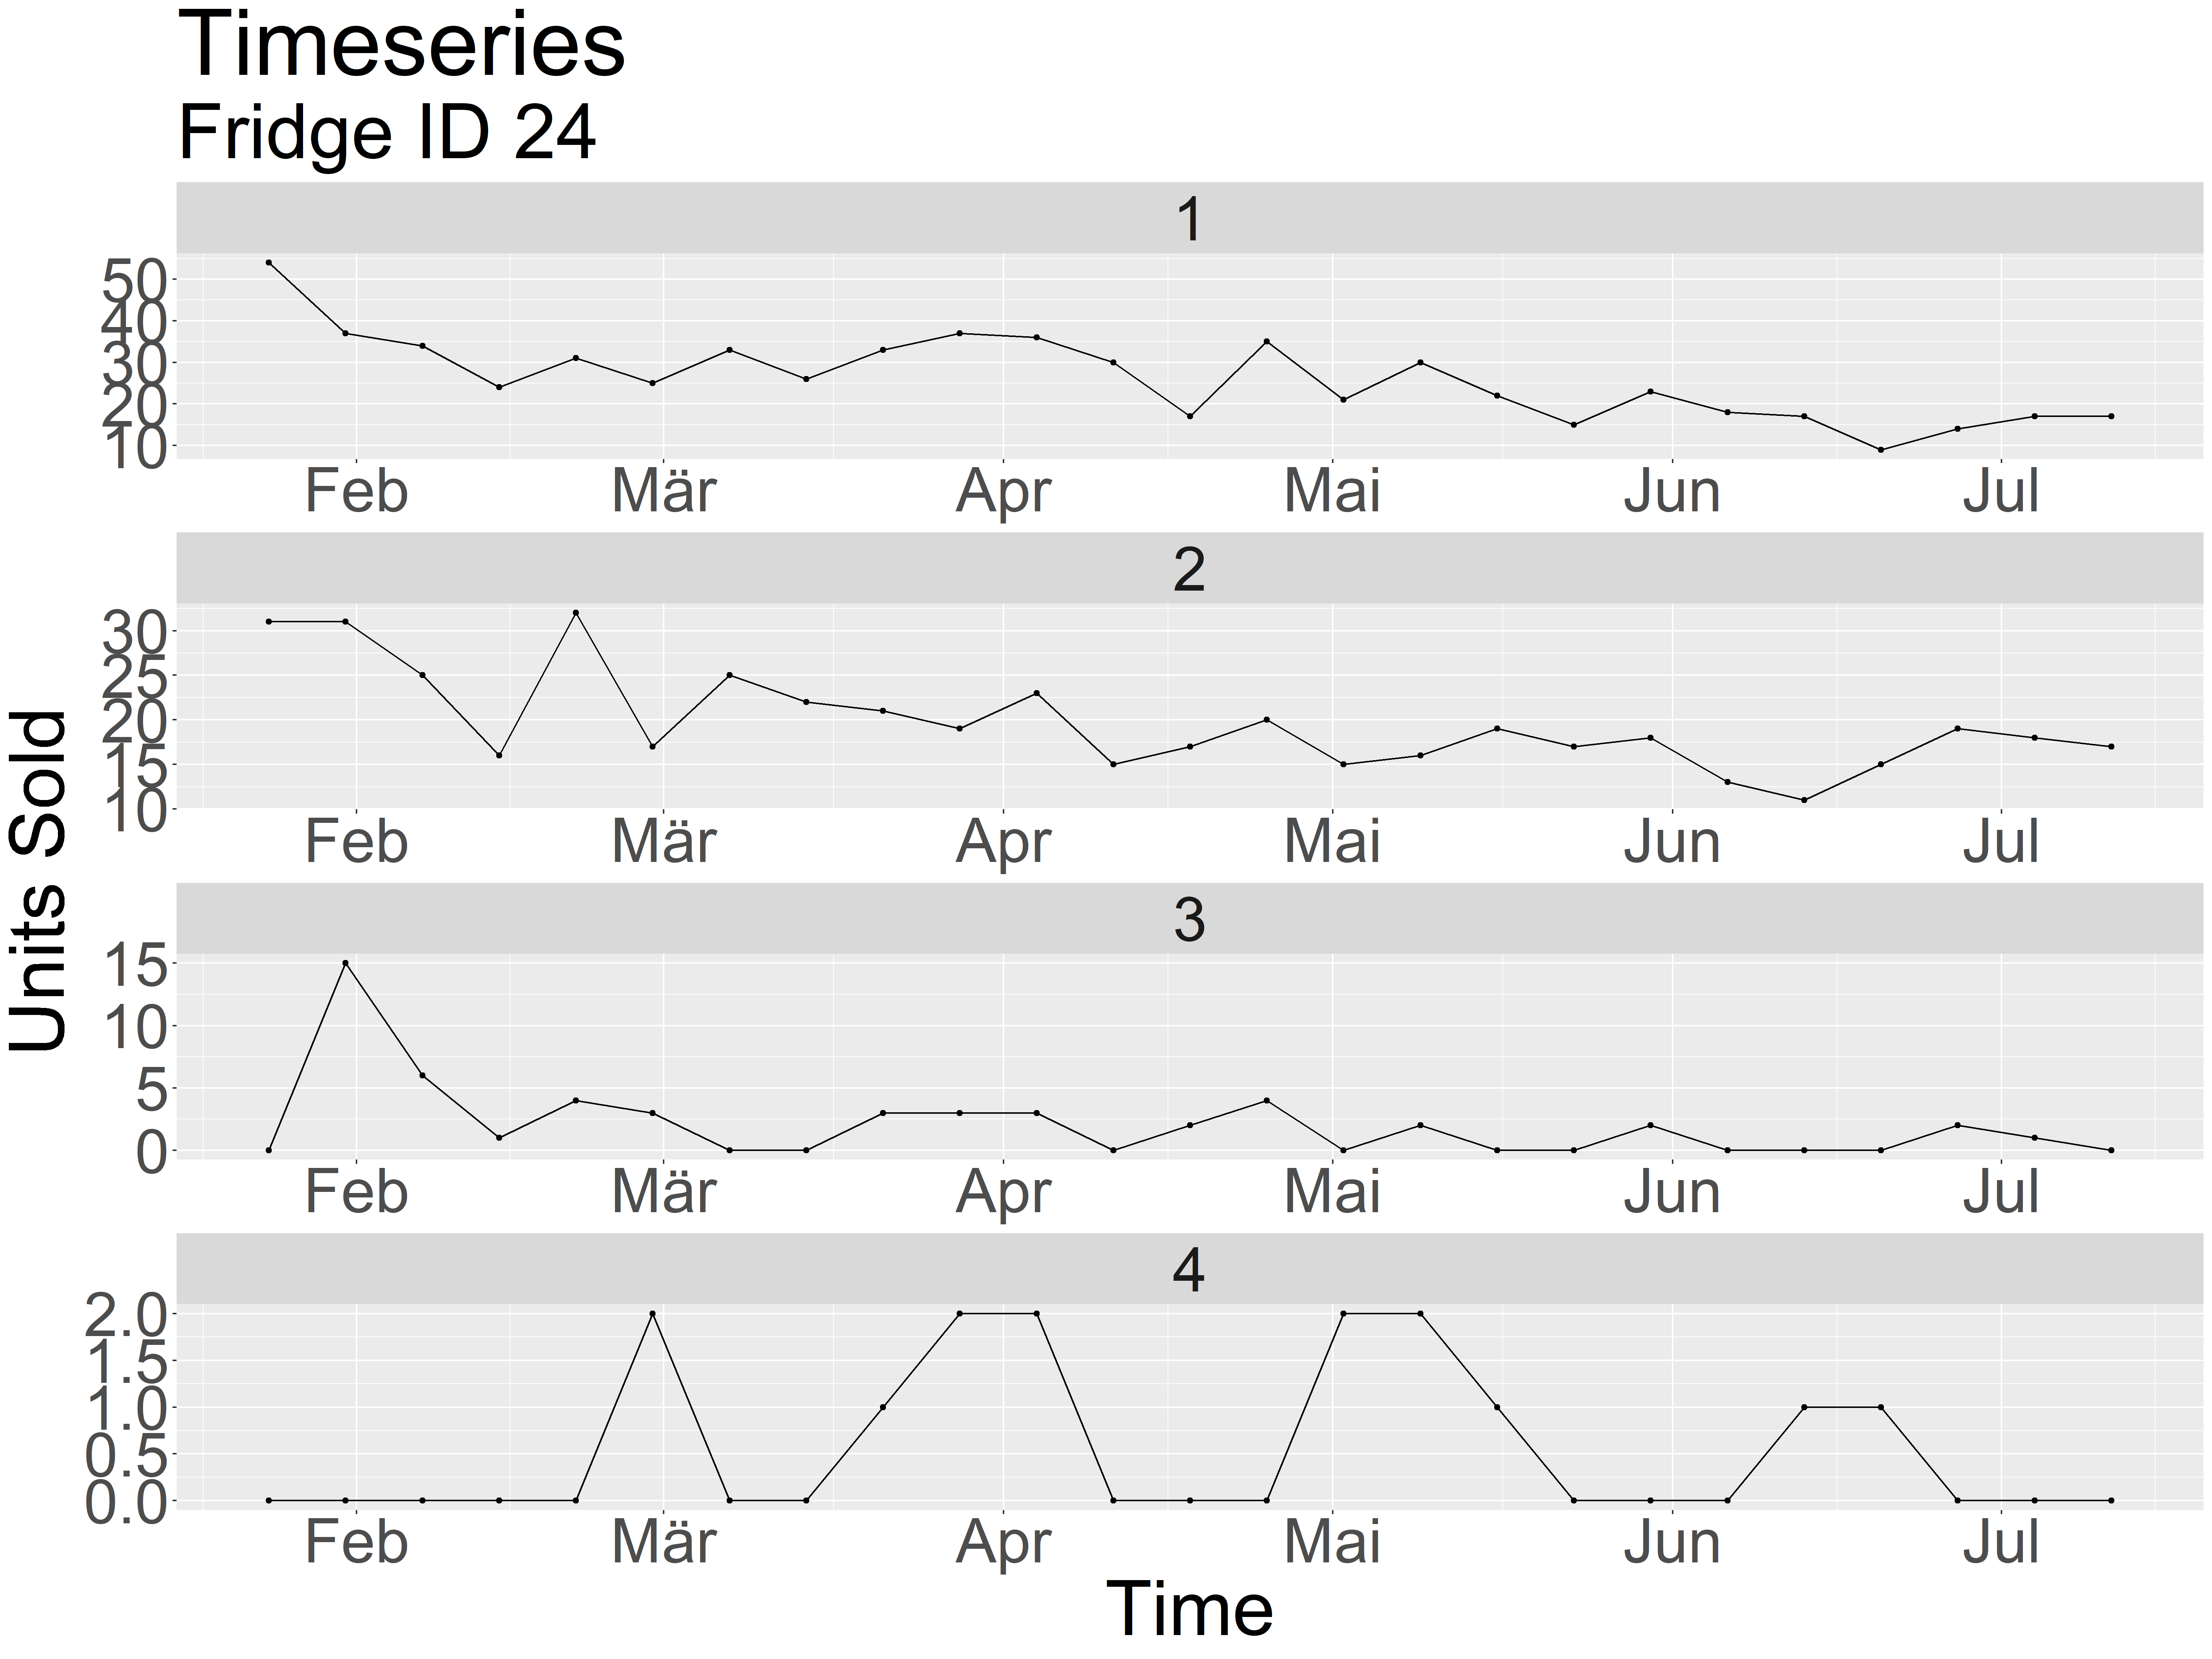
\includegraphics[width=\textwidth]{Raw_Timeseries_ID24.png} 
\caption{Fridge 24 with all four main categories}
\label{fig:TS Fridge 24}
\end{subfigure}
\caption{Time series for two fridges}
\label{fig:TS raw}
\end{figure}


The two plots in \ref{fig:TS raw} are good examples of the composition of our data. The scales of the sold units within a fridge vary widely. For example in figure \ref{fig:TS Fridge 24} the values for category 1 vary from above 50 to as low as 10, while for category 4 we only have values in the range of 0 to 2. In both figures \ref{fig:TS raw} for category 4, we can see the excessive amount of zero values in our data which makes the previously mentioned transformations necessary. 

Next in figure \ref{fig:TS Coda}, we add the predictions of the CoDA model. For this model we used the whole history and half of the data for the window length. In addition we extend the window at every time point, add 0.5 to all values and use the one-vs-all method. We can see that this captures the general trend well however, struggles with unexpected high peaks. In addition it is able to handle the difference in scales as seen in \ref{fig:Coda Fridge 4}. Both, categories 1 and 2 with bigger values and categories 3 and 4 with lower values, are in general modelled well. Also in time series with less data available, as in fridge 24 \ref{fig:Coda Fridge 24}, the model works well. Especially category 3 with its low values is predicted well. 

\begin{figure}[htb]
\centering
\begin{subfigure}[b]{0.45\textwidth}
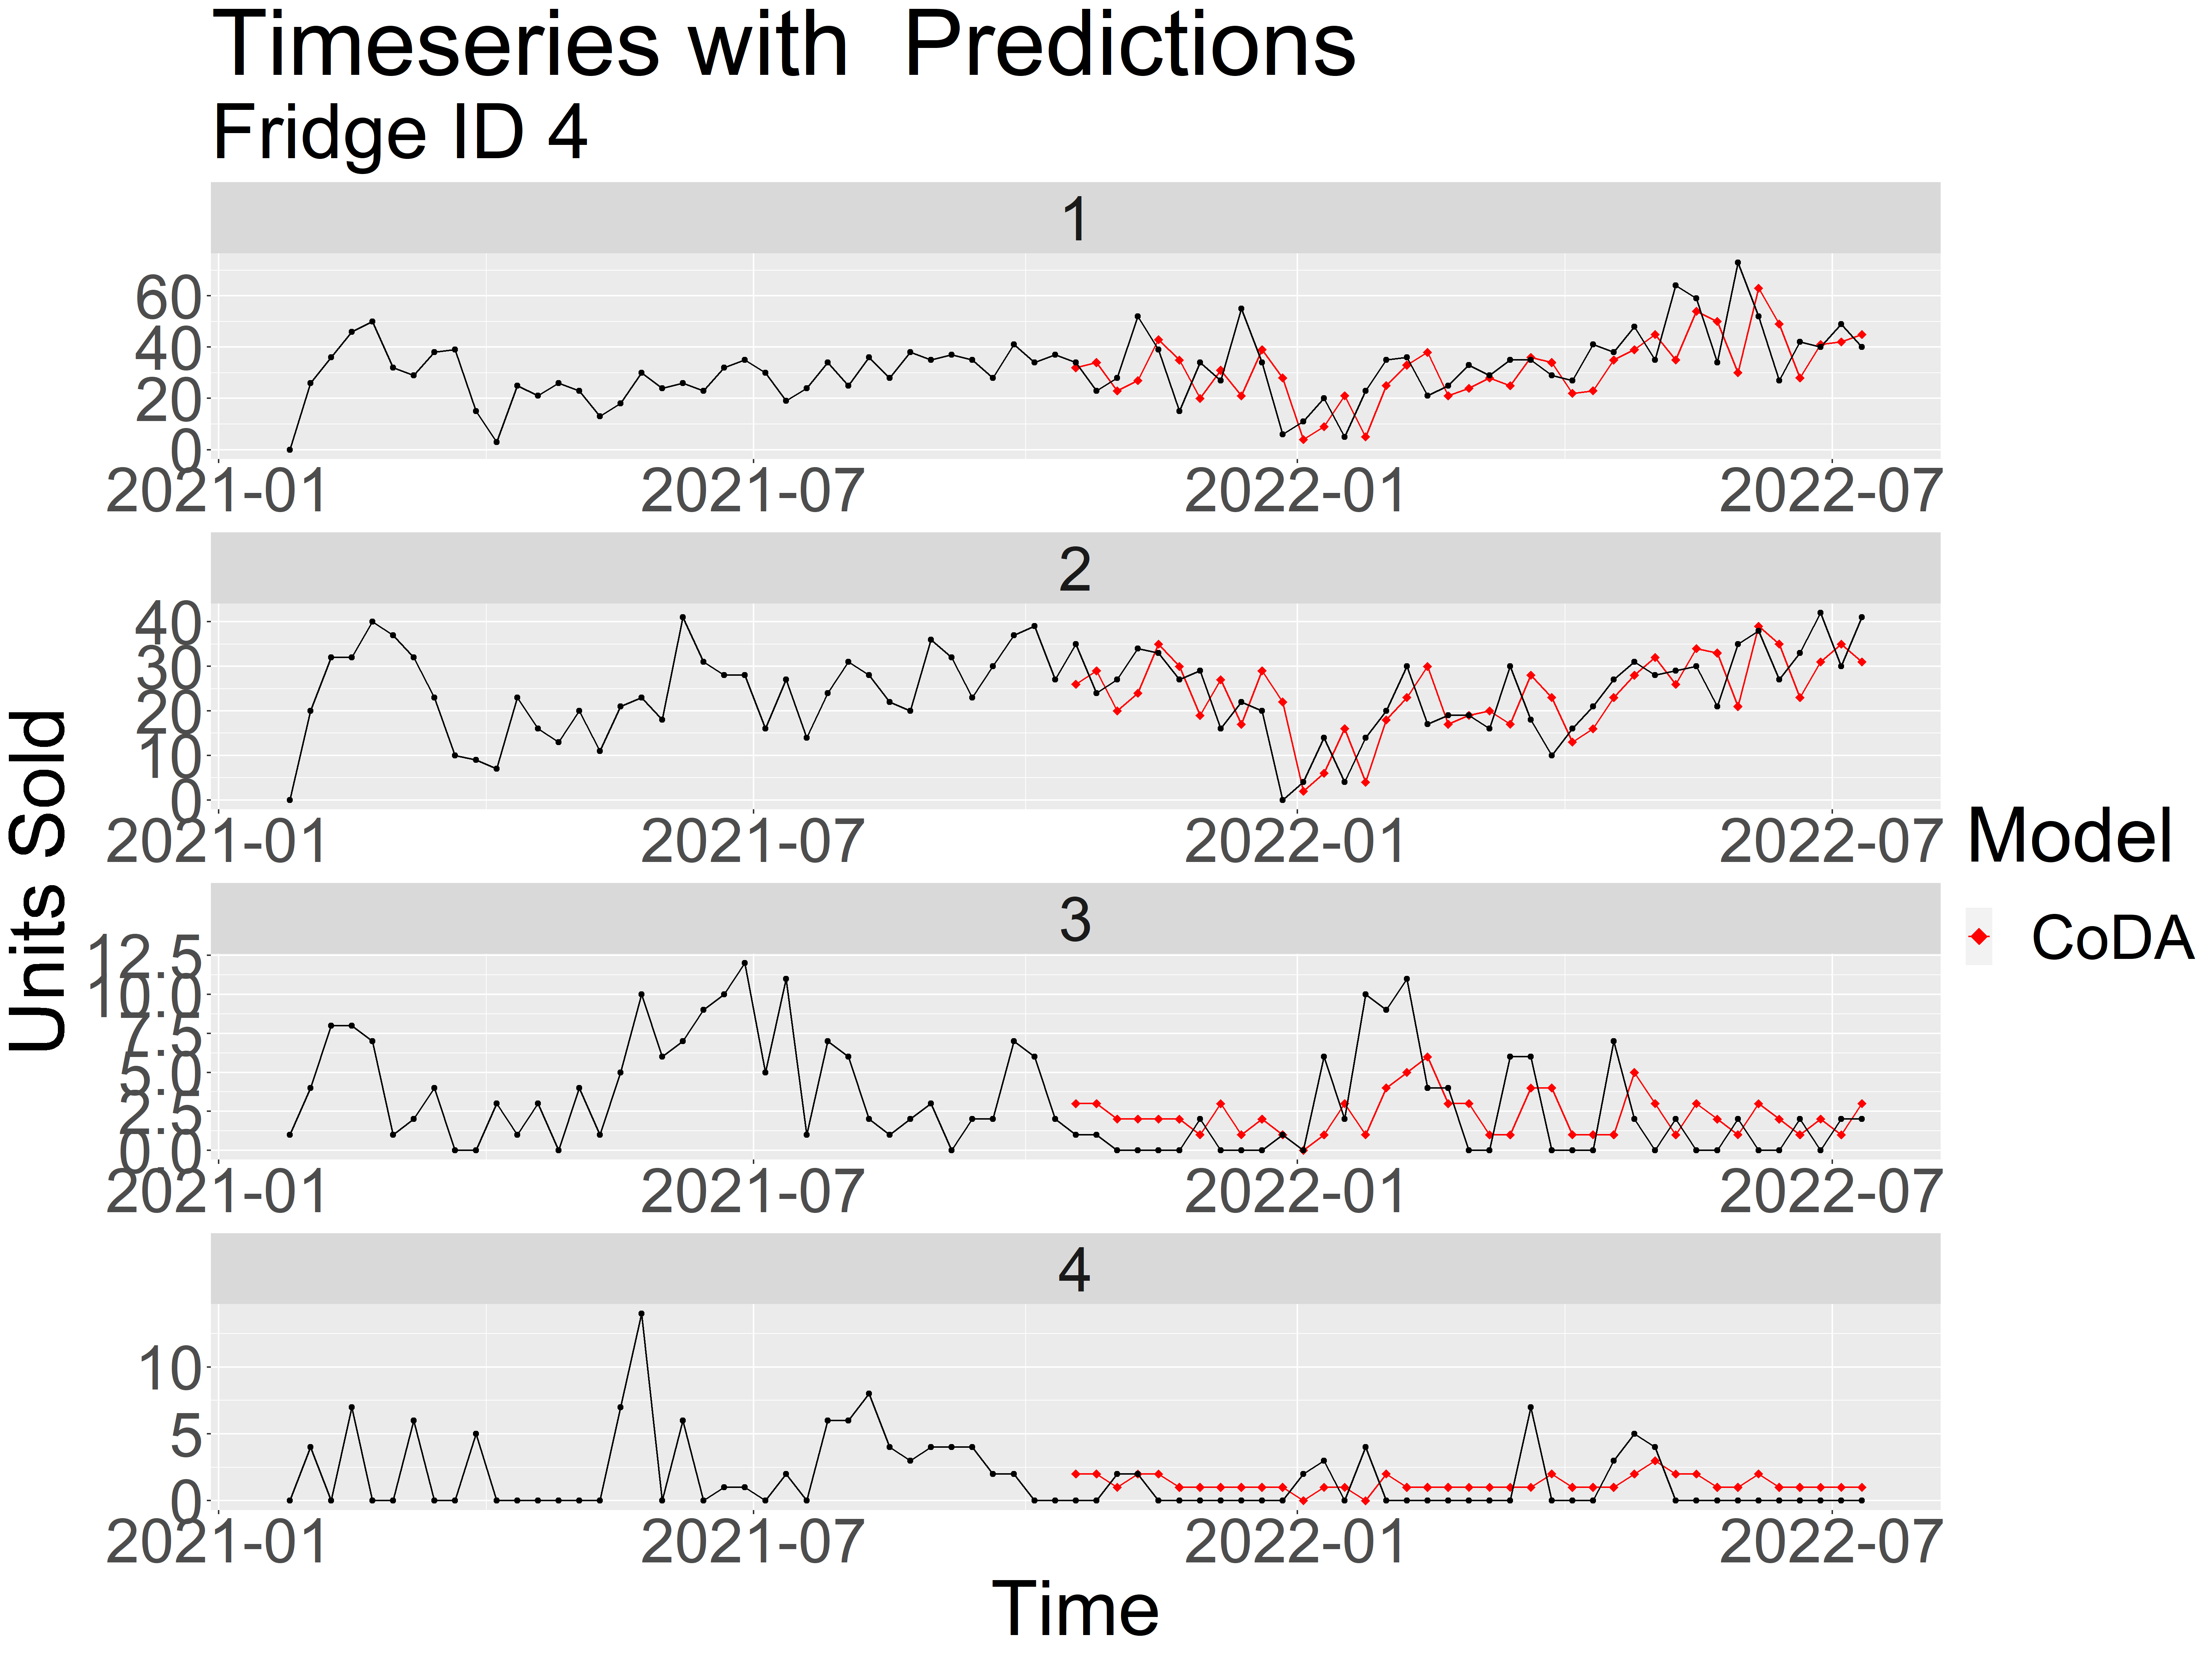
\includegraphics[width=\textwidth]{Coda_Timeseries_ID4.png}
\caption{Fridge 4 with the CoDA model}
\label{fig:Coda Fridge 4}
\end{subfigure}
\hfill
\begin{subfigure}[b]{0.45\textwidth}
\includegraphics[width=\textwidth]{Coda_timeseries_ID24.png}
\caption{Fridge 24 with the CoDA model}
\label{fig:Coda Fridge 24}
\end{subfigure}
\caption{Time series with CoDA model}
\label{fig:TS Coda}
\end{figure}

In figure \ref{fig:TS Ingarch} we apply the INGARCH model to the time series. For this, we used the whole history $T=T_F$, half of the data for the initial window length $w_f=\frac{T}{2}$, extend the window at every time point, add nothing to the zero values and used the poisson distribution. We used no external factors and set $p=1, q=1$ in model \ref{eq:Ingarch model with external effect}. The general trend is again captured well and in the instance of \ref{fig:Ingarch Fridge 4} it seems to be more reactive to sudden peaks, as often the value predicted after such a peak is heavily influenced by it.

\begin{figure}[htb]
\centering
\begin{subfigure}[b]{0.45\textwidth}
\includegraphics[width=\textwidth]{Ingarch_timeseries_ID4.png}
\caption{Fridge 4 with the INGARCH model}
\label{fig:Ingarch Fridge 4}
\end{subfigure}
\hfill
\begin{subfigure}[b]{0.45\textwidth}
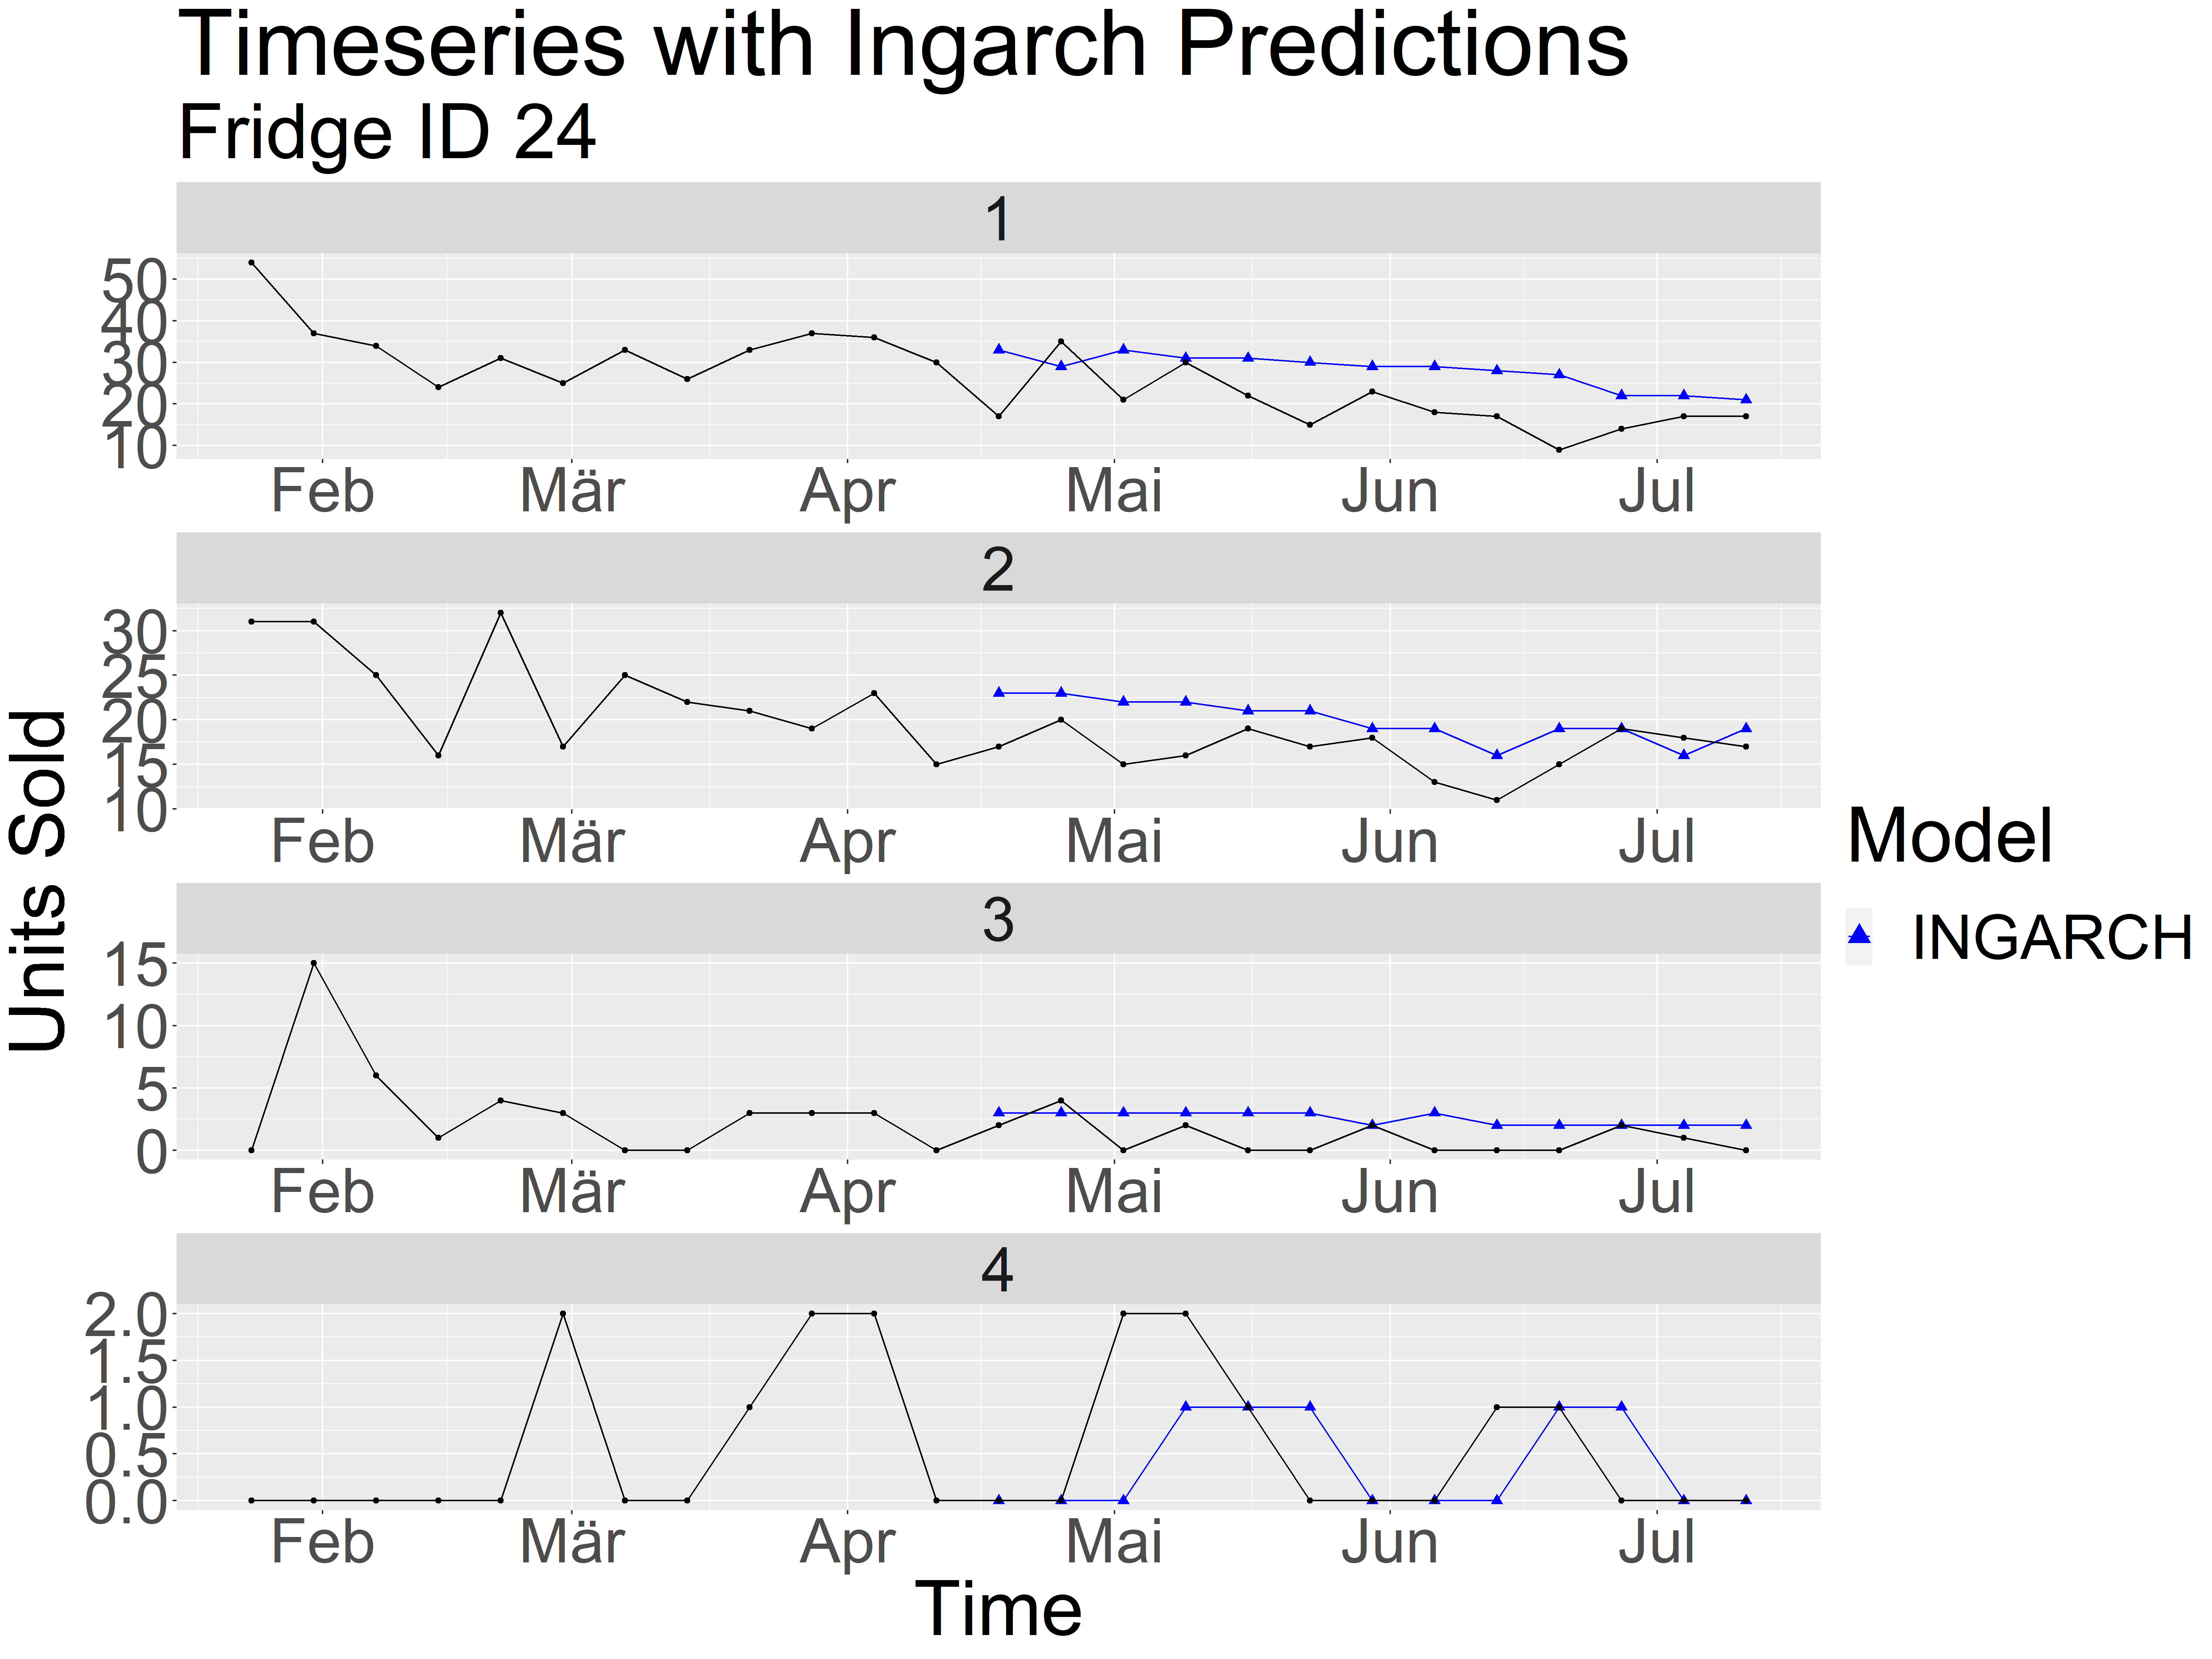
\includegraphics[width=\textwidth]{Ingarch_Timeseries_ID24.png}
\caption{Fridge 24 with the INGARCH model}
\label{fig:Ingarch Fridge 24}
\end{subfigure}
\caption{Time series with INGARCH model}
\label{fig:TS Ingarch}
\end{figure}


To directly compare both models, we plot the predictions in one figure \ref{fig:TS Both}. The model specifications are the same as above. We can see that the models produce similar results to each other. In this instances it appears that INGARCH predicts slightly higher values than CoDA. 

\begin{figure}[htb!]
\centering
\begin{subfigure}[b]{0.8\textwidth}
\includegraphics[width=\textwidth]{Both_timeseries_ID4.png}
\caption{Fridge 4 with the both models}
\label{fig:Both Fridge 4}
\end{subfigure}
\hfill
\begin{subfigure}[b]{0.8\textwidth}
\includegraphics[width=\textwidth]{Both_timeseries_ID24.png}
\caption{Fridge 24 with the both models}
\label{fig:Both Fridge 24}
\end{subfigure}
\caption{Time series with both models}
\label{fig:TS Both}
\end{figure}


In order to get some further insight in the accuracy of our predictions, we added 95 \% prediction intervals \ref{fig:TS BothPI}. Here we can see some differences between the intervals. While for categories with bigger values the bands are quite similar in width, for categories with lower values, CoDA has much wider bands. This is especially visible in \ref{fig:BothPI Fridge 4} for category 3 and 4. However, most data points are covered by both bands.
\begin{figure}[htb!]
\centering
\begin{subfigure}[b]{0.8\textwidth}
\includegraphics[width=\textwidth]{BothPI_timeseries_ID4.png}
\caption{Fridge 4 with the both models and their prediction intervals}
\label{fig:BothPI Fridge 4}
\end{subfigure}
\hfill
\begin{subfigure}[b]{0.8\textwidth}
\includegraphics[width=\textwidth]{BothPI_timeseries_ID24.png}
\caption{Fridge 24 with the both models and their prediction intervals}
\label{fig:BothPI Fridge 24}
\end{subfigure}
\caption{Time series with both models and their prediction intervals}
\label{fig:TS BothPI}
\end{figure}